\section{Memory-Based Collaborative Filtering Recommender System}
As was pointed out in the formulation of this report, memory-based collaborative filtering makes recommendations based on the similarity between the users or the items. The detailed steps of the memory-based collaborative filtering can be stated as follows:
\begin{itemize}
    \item[1. ]Identify a target user who will be recommended.
    \item[2. ]Figure out the items that the target user has given ratings for.
    \item[3. ]Based on the target user’s rating pattern, find similar users.
    \item[4. ]Get the rating records of similar users for items.
    \item[5. ]Calculate the similarity between the target user and a similar user by formula (e.g., \textit {Euclidean Distance}, \textit{Pearson Correlation}, \textit{Cosine Similarity}).
    \item[6. ]Recommend the items with the highest score to the target user.

\end{itemize}
In the following, an example will be demonstrated to elaborate on the above steps.
\begin{figure}[htbp]
\centering
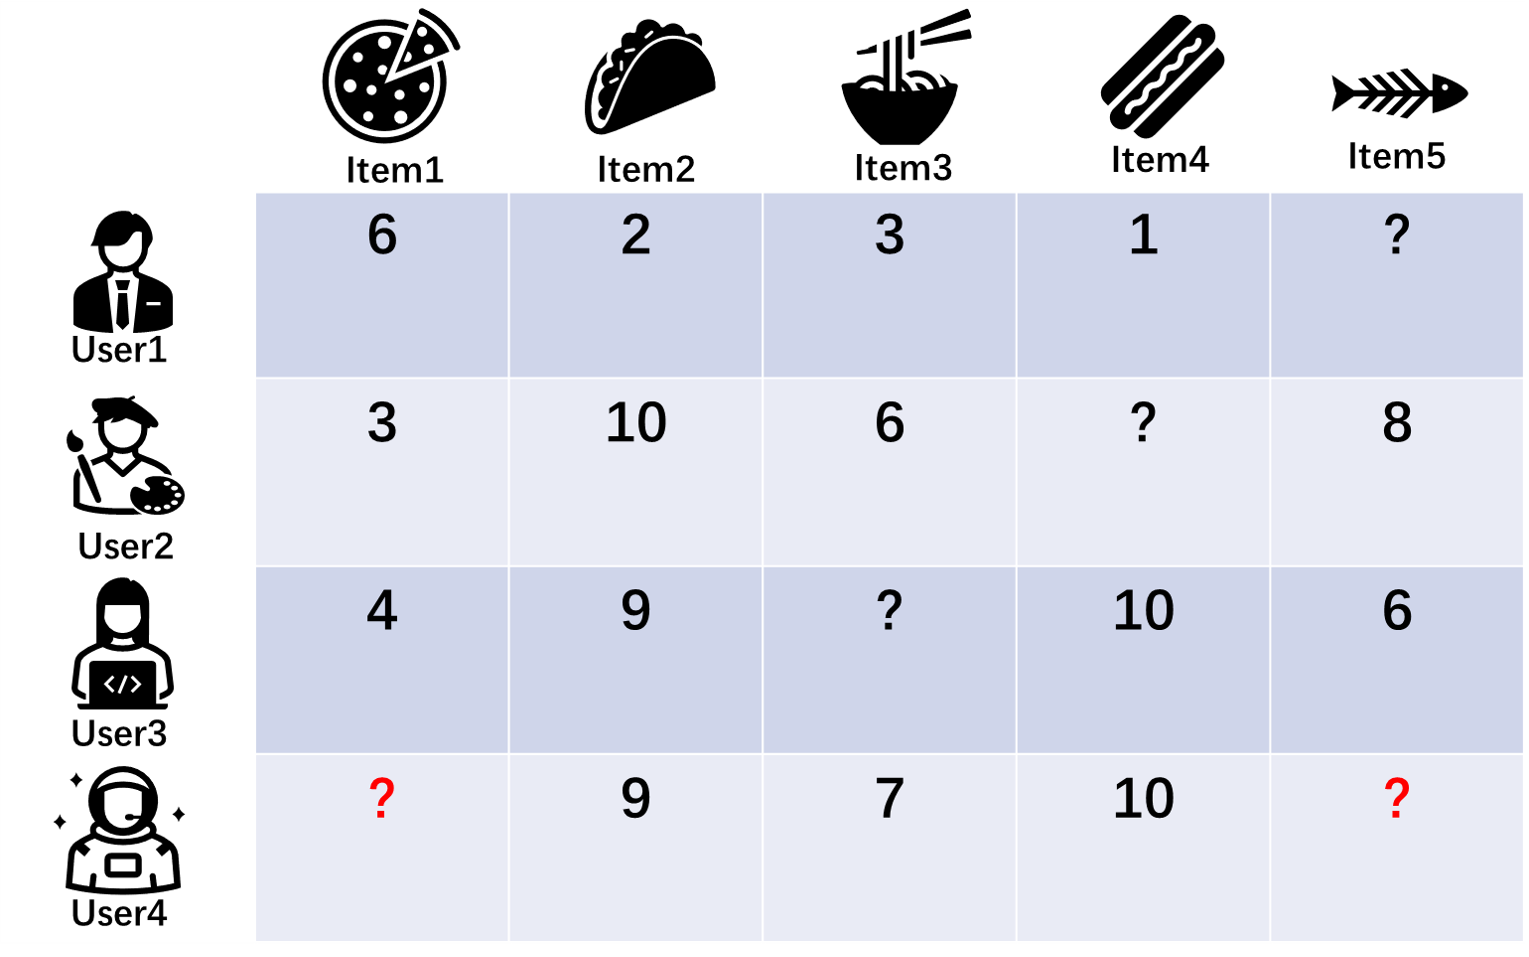
\includegraphics[scale=0.55]{figure/rating1.png}
\caption{Example of User$-$item rating matrix}
\end{figure}

As per the user-item rating matrix shown in Figure 3.1, assume \textit{user4} is our target user and rated three out of five items. The goal of the system is to figure out which one of the two unrated items (i.e., \textit{item1} and \textit{item5}) should be recommended to the target user who can probably get a high rating. After we define our target user and figure out some users, the next step that comes up is to calculate the similarity between the target user and similar users. The common methods of similarity calculation include \textit{Euclidean Distance}, \textit{Pearson Correlation}, \textit{Cosine Similarity}. To calculate the similarity between two users, we base it on the ratings of \textit{item2}, \textit{item3}, and \textit{item4} which are the items that all users have rated.
\begin{figure}[htbp]
\centering
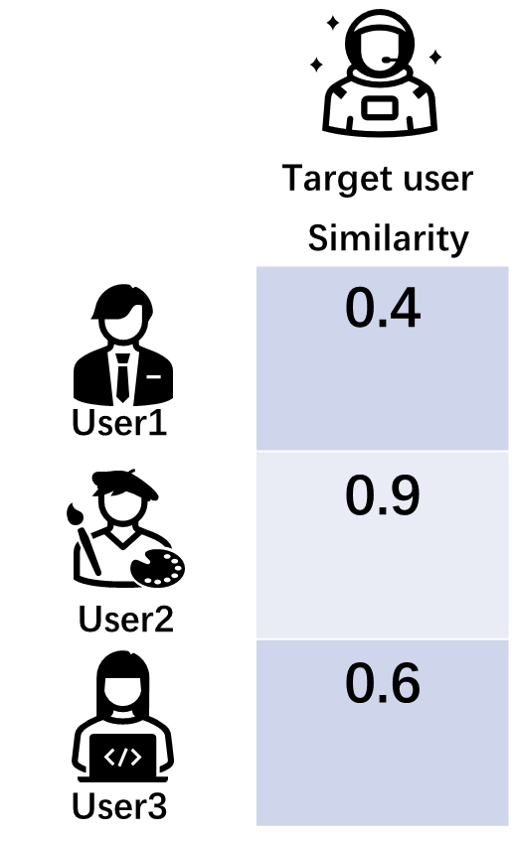
\includegraphics[scale=0.5]{figure/rating2.png}
\caption{Similarity between target user and other users}
\end{figure}
Here we make a hypothesis that the similarity between the target user and other users is 0.4, 0.9, and 0.6, respectively, as shown in Figure 3.2. The next step is that, based on the value of similarity, we can calculate the predicted rating for the target user. What can be seen in Figure 3.3 is the so-called weighted rating matrix because it provides more weight to those users who have a higher similarity to the target user.
\begin{figure}[htbp]
\centering
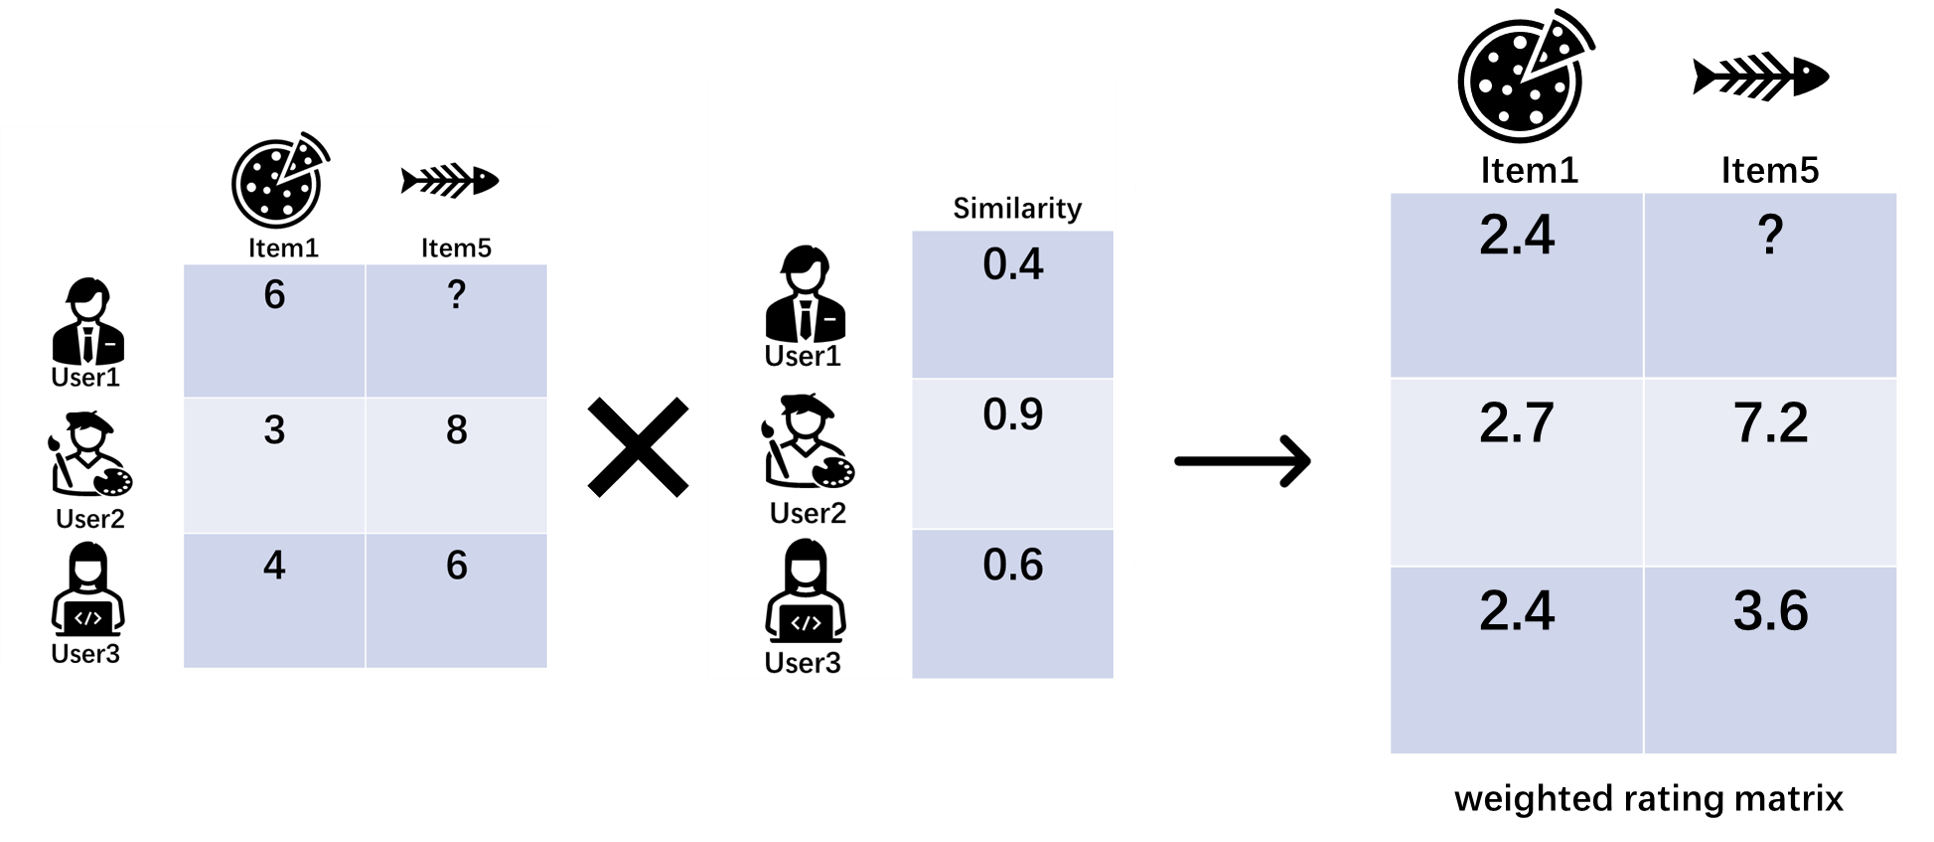
\includegraphics[scale=0.5]{figure/rating3.png}
\caption{Weighted rating matrix}
\end{figure}
For the final step, we tally up all weighted rates to create the recommender matrix. Due to the sparsity of the weighted rating matrix (e.g. only \textit{user2} and \textit{user3} provided the rating for \textit{item5} , we normalize the value of the weighted rating by dividing the sum of weighted ratings by the sum of the similarity for users.
\begin{figure}[htbp]
\centering
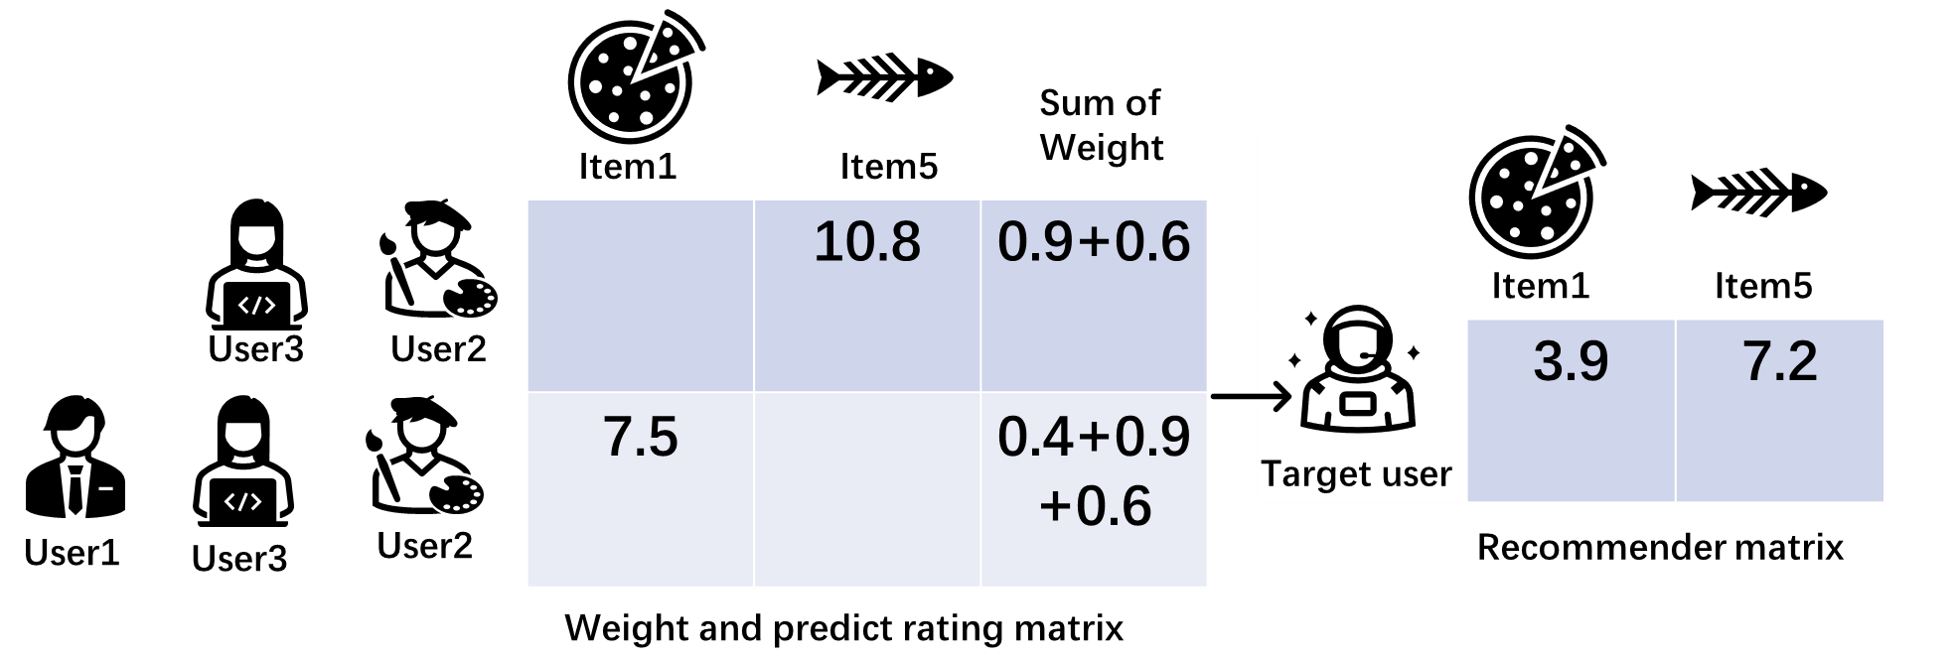
\includegraphics[scale=0.5]{figure/rating4.png}
\caption{Recommender matrix}
\end{figure}
According to the result of user-based collaborative filtering shown in Figure 3.4, the value in the recommender matrix describes the potential rating for the target user that will arise for the items based on the similarity between them and other users. The target user potentially provides a higher rating to \textit{item5} than \textit{item1}. So, through the result, the user-based collaborative filtering recommender system will choose \textit{item5} to recommend to the target user.